\documentclass[10pt,a4paper]{report}
\usepackage{graphicx}
\usepackage{float}
\usepackage[utf8]{inputenc}
\usepackage[top=3cm, bottom=3cm, left=3cm, right=3cm]{geometry}

%opening
\title{TP rapport Master 2 Images}
\author{GRIVOLLAT Aurélien, MALVEZIN Kevin}
\date{2 décembre 2014}

\begin{document}

\maketitle

\chapter{Introduction}

\hspace*{10mm} Le but de ce projet est de construire un maillage par triangulation selon le principe de Delaunay d'un terrain 2D 1/2 à partir de données altimétriques. 
	\newline \newline
\hspace*{10mm}Afin d'apporter une personnalisation à l'utilisateur, nous avons passé plusieurs valeurs en paramètres. La quantité de points insérés, le nombre de facettes créées et le niveau d'adéquation du maillage du terrain en fonction d'un ou plusieurs paramètres passés en entrée sont autant de critères d'arrêt.
	\newline\newline
\hspace*{10mm}Nous offrons aussi à l'utilisateur la possibilité de voir le maillage en deux dimensions et en trois dimensions. Avec cela s'ajoute deux lancements différents. Le lancement complet créé tout le maillage et affiche une fois les calculs effectués. Le pas à pas montre la construction visuel du maillage d'ajout de point par ajout de point.
Nous allons présenter ici le travail effectué sur ce projet, ainsi que les choix algorithme qui ont été mis en place.

\chapter{Structure}

	\section{Structure de représentation}
	
\hspace*{10mm}Lors de ce projet nous avons mis en place plusieurs structures:
\newline\newline
		%\subsection{Vertex}
\hspace*{10mm}La structure $\it{vertex}$ stocke toutes les informations pour la représentation d'un point, c'est à dire ces coordonnées dans les dimensions voulues. Ici nous avons besoin des trois premières dimensions.
\newline \newline
		%\subsection{Simplex}
\hspace*{10mm}La structure $\it{simplex}$ permet de stocker toutes les informations nécessaires à la création d'un triangle dans le maillage. Il contient les trois vertex qui le représentent, le lien vers ses trois voisins dans le maillage, les points que l'on va appeler “candidats”, qui sont les points dont le projeté appartient au simplex, son équation du plan, ainsi qu'une valeur de hauteur qui sera expliqué plus tard dans le projet.

	\section{Structure de stockage}
		
\hspace*{10mm}Nous avons aussi construit de nouvelles structures de stockage afin d'améliorer le temps d'exécution et la facilité d'utilisation et de gestion des informations.
\newline \newline		%\subsection{File}
\hspace*{10mm}Nous avons créé une $\it{file de priorite}$ sur les simplex qui nous permet en tout temps d'avoir l'ensemble des simplex qu'elle contient, triés par rapport à la valeur hauteur du simplex. Cette valeur de hauteur représente la hauteur verticale maximum des points candidats de ce simplex par rapport à ce même simplex. Chaque ajout de simplex entraîne une remise en forme de la file pour conserver son ordre.		
\newline \newline		%\subsection{Pile}
\hspace*{10mm}La $\it{pile}$ est un espace que l'on a voulu simple, le premier entré est le premier sorti, on trie donc les informations contenue dans la pile, par leur ordre d'arrivée.
\newline \newline		%\subsection{Liste}
\hspace*{10mm}La $\it{liste}$ sert à stocker des vertex, un accès au début et à la fin de la liste permet d'ajouter facilement les vertex par importance. C'est à dire, un vertex que l'on juge plus important que ceux déjà dans la liste est ajouté au sommet, les autres en queue. Bien sur, seul le premier élément de cette liste à une importance dans ce cas.
		
\chapter{Création du maillage}
	
	\section{Initialisation}
\hspace*{10mm}La première étape consiste à générer les points du maillage. Autrement dit, pour n points, si on veut appliquer l'algorithme de Delaunay, il faut qu'au moins quatre de ces points soient situés aux extrémités du maillage, soit aux coordonnées [0,0], [0,1], [1,0], [1,1]. Leurs coordonnées altimètrique sont choisis aléatoirement. Les autres points créés seront donc situés dans le carré formé par ces quatre points. 
La mise en place de la file de priorité va permettre de mettre un ordre sur les simplex à traiter en premier. Le premier simplex est donc celui avec la hauteur verticale de son candidat supérieur à celle de tous les candidats des autres simplexes. Il faut également initialiser une pile. La pile et la file seront toutes deux de taille 2*n-6. La pile va stocker les simplex en attente de changement de diagonale (nous expliquons cette opération plus tard dans le rapport). La liste quand à elle est utilisée dans chaque simplex pour stocker l'ensemble des vertex candidats.
\newline \newline
\hspace*{10mm}On commence donc par créer les deux premiers simplex, à partir des quatre premiers vertex du tableau : les quatre vertex frontières du maillage. On distribue ensuite les autres vertex candidats entre les deux simplex : on fait la projection de ce vertex et du simplex sur un même plan, et on vérifie si l'un est contenu dans l'autre (si le vertex est sur l'un des segments, on le considère comme inclut). \newline
Les vertex sont alors triés dans une liste triée : seul le plus haut est au sommet de la pile. Nous avons donc, pour chaque simplex construit, son vertex candidat le plus haut. On peut alors mettre ces simplex dans la file de priorité, qui les trie par hauteur.

	\section{Boucle de l’algorithme}
\hspace*{10mm}On va commencer par récupérer, et donc retirer de la file de priorité, le simplex contenant le “plus grand” vertex candidat (par rapport à sa hauteur verticale). on divise alors ce simplex en trois nouveaux simplex à partir de ce nouveau vertex. 
On redistribue alors les vertex candidats entre ces trois simplex, puis l'on modifie le voisinage.
	
\begin{figure}[!htbp]
	\begin{center}
  		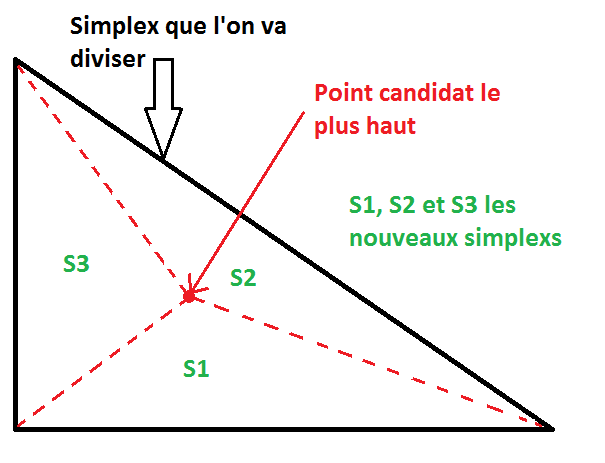
\includegraphics[scale=0.5]{Division3Simplex.png}
  		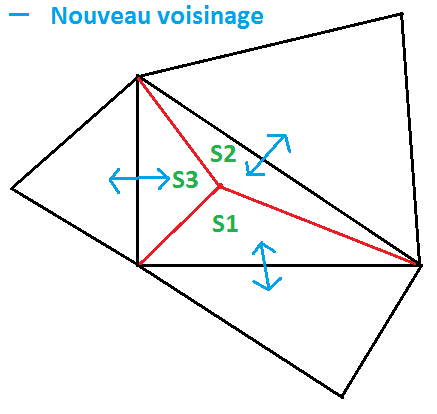
\includegraphics[scale=0.5]{Division3SimplexVoisin.png} 
  	\end{center}
   	\caption{Illustration de la division d'un simplex}
	\label{Illustration de la division d'un simplex}
\end{figure}


On empile ensuite ces simplex, dans la pile précédemment créée pour les éléments en attente de flip de diagonale. L'ordre n'a pas ici d'importance, tous les éléments de la pile vont être traités avant le prochain ajout de point..
\newline \newline
\hspace*{10mm}On arrive donc à la partie importante de cet algorithme, le moment où l'on doit traiter les possibles cas d'inversion de diagonales. En effet, dans un maillage, il est préférable que les mailles entre les points soient les plus courtes possibles, pour respecter le principe de delaunay, et pour une meilleure appréciation visuelle. Ainsi, à chaque empilement de nouveau simplex, il est important de vérifier le principe de Delaunay : 
On dépile donc le premier simplex de la pile et l'on va tester pour chacun de ces voisins, qui n'est pas déjà présent dans la file, si il peut y avoir un inversement de diagonale. Pour cela nous avons besoin de tester si le simplex et son voisin sont convexes comme le montre les illustrations ci dessous:

\begin{figure}[h]
	\begin{center}
  		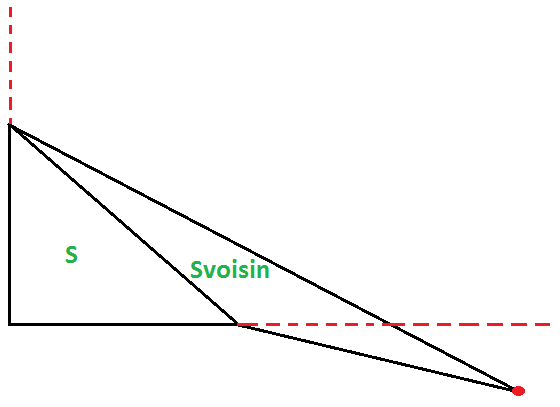
\includegraphics[scale=0.5]{DivisionDiagImpossible.png} 
  		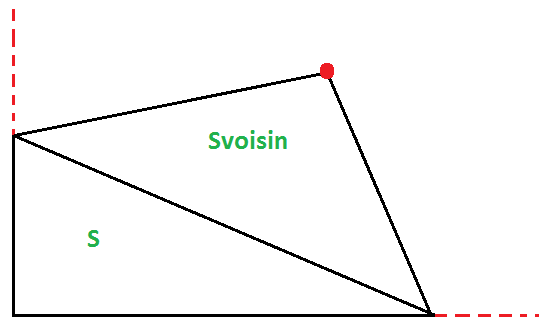
\includegraphics[scale=0.5]{DivisionDiagPossible.png} 
  	\end{center}
   	\caption{Illustration non convexe et convexe}
	\label{Illustration non convexe}
\end{figure}


\hspace*{10mm}Il se peut que les deux simplex en cours de traitement ne puissent changer de diagonales, car l'ensemble des quatre vertex qui les définissent tout deux n'est pas convexe. Dans ce cas là, on regarde les autres voisins afin de vérifier qu'il n'y ai pas de meilleurs candidats. Si malgré tout il n'y pas pas d'ensemble convexe avec ses voisins, ce simplex ne peut pas changer sa diagonale, on passe donc au prochain simplex de la pile.
Si l'on rencontre enfin un élément dont la convexité est vérifié, il reste une étape avant d'inverser sa diagonale. Il nous faut tester à l'aide du cercle circonscrit. \newline
On forme à l'aide des point du simplex, le cercle circonscrit. Si le point du voisin n'appartenant pas au simplex est dans ce cercle, on inverse les diagonales, dans le cas contraire pas d'inversion nécessaire, on passe donc à l'élément de la pile suivant.

\begin{figure}[h]
	\begin{center}
  		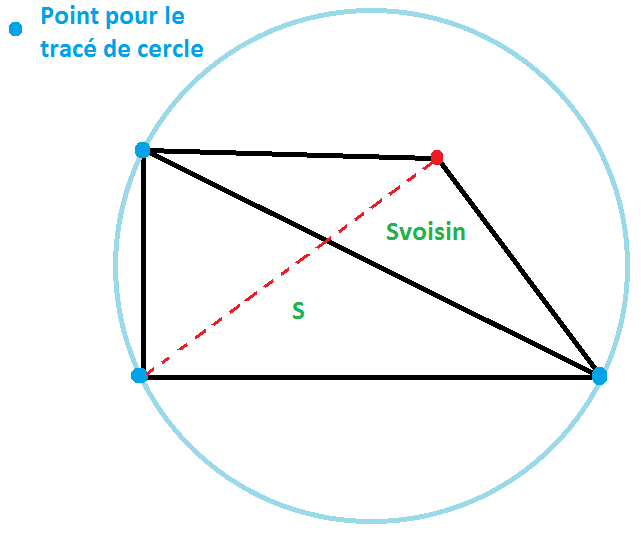
\includegraphics[scale=0.5]{DivisionDiagPossibleCercle.png} 
  	\end{center}
   	\caption{Illustration du cercle circonscrit}
	\label{Illustration du cercle circonscrit}
\end{figure}

Si toutes les tests d'inversement de diagonale sont vérifiés, on modifie alors les simplex. On redistribue les vertex candidats dans les deux nouveaux simplexes puis on redéfinie les voisins.

\begin{figure}[h]
	\begin{center}
  		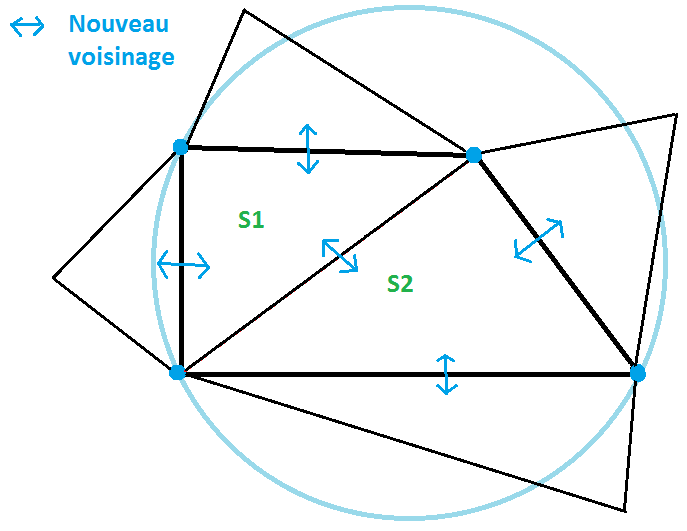
\includegraphics[scale=0.5]{DivisionDiagPossibleCercleApres.png} 
  	\end{center}
   	\caption{Illustration du flip de diagonale}
	\label{Illustration du flip de diagonale}
\end{figure}

\hspace*{10mm}On empile ces deux nouveaux simplex pour tester d'éventuels nouveaux changement de diagonales avec leurs nouveaux voisins. Puis on les rajoute dans la file de priorité.
\newline
Pour bien comprendre, il faut garder à l'esprit que la file de priorité gère les simplex qui ont encore des points candidats, alors que la pile contient les simplex qui sont en attentes de possible changement de diagonale. 
\newline
On recommence l'algorithme tant qu'il y a des simplex dans la file de priorité. Si celle-ci est vide, cela signifie que tout les points ont été distribuées.

\chapter{Affichage}
	
\hspace*{10mm}Construire un maillage c'est bien, pouvoir le visualiser c'est mieux.
Afin de vérifier la bonne corrélation des résultats, il est nécessaire de construire un environnement graphique. On se sert ici de la bibliothèque OpenGL, qui permet de mettre en place une fenêtre de visualisation, et d'interagir avec.  \newline \newline
Dans un premier temps, il s'agit de dessiner les vertex et les simplex. Une simple fonction d'affichage $\it{display()}$ convient parfaitement, avec à l'intérieur deux boucles bien distinctes : une pour les points, d'une certaine couleur, l'autre pour les lignes les reliant, d'une couleur différente. Cela ajoute une lisibilité certaine à la lecture du maillage. On peut également, avec une option en entrée du programme, choisir entre un mode de dessin direct, ou un mode pas à pas, qui va dessiner les simplex formés les uns après les autres, mais cela implique de pouvoir interagir avec la fenêtre. \newline 
OpenGL fournit pour ça deux méthodes : $\it{glutKeyboardFunc()}$ et $\it{glutDisplayFunc()}$, qui vont chacune prendre le nom d'une procédure en entrée. Cela revient à indiquer à OpenGL quelle méthode nous souhaitons utiliser, soit pour dessiner, soit pour interagir, ici avec le clavier. Ainsi, au sein de notre méthode d'interaction, on peut designer une toucher servant à débloquer un tour de boucle de l'algorithme, et voir sa progression sur l'écran.

\begin{figure}[h]
	\begin{center}
  		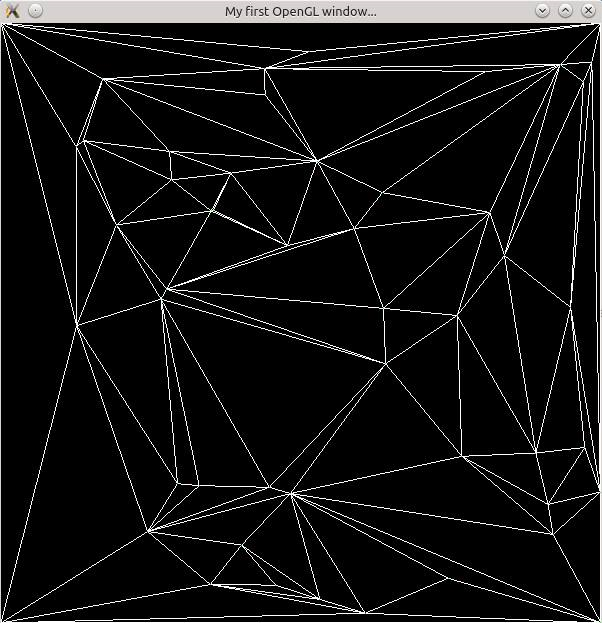
\includegraphics[scale=0.5]{2D.png} 
  	\end{center}
   	\caption{Illustration de l'affichage 2D}
	\label{Illustration de l'affichage 2D}
\end{figure}

\chapter{Contraintes}

\hspace*{10mm}Ce projet s'accompagnait de plusieurs contraintes : la possibilité de limiter le nombre de facettes du maillage ou de choisir entre une vue 2D du dessus, ou une vue 3D capable d'évoluer autour du maillage.
Pour le nombre de facette maximum du maillage, il est nécessaire de rajouter une contrainte à chaque début de la boucle de l'algorithme, testant si le nombre de simplex à afficher, donc ceux déjà traités, est bien inférieur au nombre de facettes demandé.\newline
Pour une vue en 3D, c'est un peu plus compliqué. Il est en premier temps obligatoire de définir de nouvelles méthodes de dessin et d'interaction avec la fenêtre.\newline 
Pour la nouvelle méthode $\it{displaySimplex3D()}$, on commence par initialiser la matrice de modèle-vue, grâce à laquelle on va pouvoir influencer sur le dessin suivant les mouvements de la caméra. Ensuite, on sépare la procédure d'affichage du simplex en deux : une pour les lignes, et l'autre pour le triangle.\newline 
Avec la méthode $\it{glPolygonMode()}$, on peut dessiner les triangles d'une certaine couleur, et ensuite leurs limites d'une autre, pour un meilleur rendu. De plus, en activant $\it{glEnable(GL_DEPTH_TEST)}$, on est sur de ne dessiner que les objets visibles par la caméra. \newline
La nouvelle méthode d'interaction va, elle, implémenter de nouvelles touches pour contrôler la caméra : six pour les transitions et six pour les rotations. \newline
A chaque pression, on incrémente ou décrémente le tableau de trois valeurs associé, que l'on passe en une fois à $\it{glRotatef()}$ ou $\it{glTranslatef()}$. Ainsi, le repère de l'image n'est pas déplacé et les divers déplacements de la caméra n'en sont pas affectés. \newline


Nous n'avons pas pu mettre en place la contrainte sur le seuil de hauteur pour les points candidats d'un simplex au cours de ce projet.

\chapter{Conclusion}
	\hspace*{10mm}Le projet fonctionne et le principe de Delaunay est appliqué. Il est cependant nécessaire de constater certains défauts dans l'application, comme certains trous dans le maillage qui apparaissent puis disparaissent en mode pas-à-pas, même si au bout du compte, le résultat final est conforme aux attentes. Ce projet à été intéressant mais difficile sur certains points, notamment pour comprendre et appliquer au mieux le principe de Delaunay. \newline
Notre solution, si elle présente certains défauts, n'en reste pas moins un travail en étroite collaboration qui a permis à l'un comme à l'autre de progresser.

\begin{figure}[h]
	\begin{center}
  		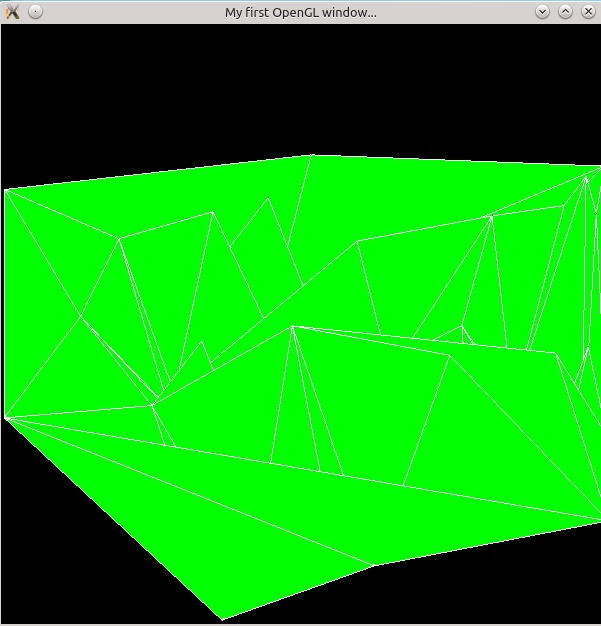
\includegraphics[scale=0.5]{3D.png} 
  	\end{center}
   	\caption{Illustration de l'affichage 3D}
	\label{Illustration de l'affichage 3D}
\end{figure}

\end{document}














